\begin{comment}
\section{\ac{MNIST} Handwritten Numbers Dataset}
\begin{figure}[H]
        \begin{center}
	    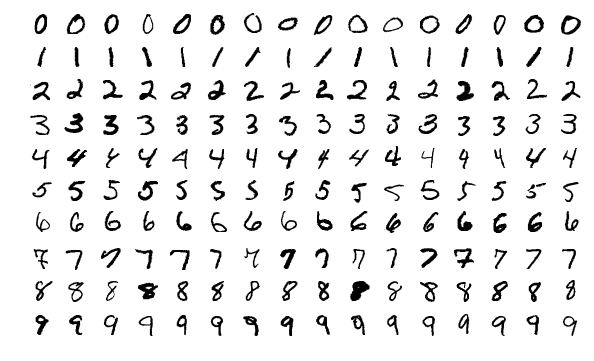
\includegraphics[scale=0.40]{images/Appendix/handwrittenCrops.png}
	    \caption[Examples of Handwritten Numbers from the \ac{MNIST} Dataset.]{Examples of Handwritten Numbers from the \ac{MNIST} Dataset.\footnotemark}
	    \label{fig:handwrittenCrops}
	    \end{center}
\end{figure}
\footnotetext{\url{http://yann.lecun.com/exdb/mnist/} last access: \dcdate}


\section{IAM Handwriting Database}

\begin{figure}[H]
        \begin{center}
	    
\includegraphics[scale=0.40]{images/Appendix/iamDataset.png}
	    \caption[Example handwritten crops from IAM handwriting database.]{Example handwritten crops from IAM handwriting database.\footnotemark}
	    \label{fig:iamDataset}
	    \end{center}
\end{figure}
\footnotetext{\url{https://fki.tic.heia-fr.ch/databases/iam-handwriting-database} last access: \dcdate}


\section{\ac{CycleGAN} Models Training}
\begin{figure}[H]
  \centering
  \begin{minipage}[b]{0.49\textwidth}
    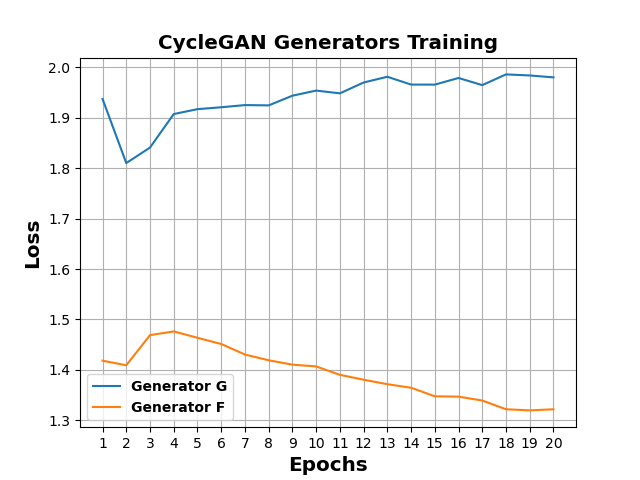
\includegraphics[width=\textwidth]{images/Evaluation/CycleGANGeneratorsTraining.png}
    \caption[\ac{CycleGAN} generators $G$ and $F$ training epochs vs loss plot.]{\ac{CycleGAN} generators $G$ and $F$ training epochs vs loss plot.}
    \label{fig:CycleGANGeneratorsTraining}
  \end{minipage}
  \hfill
  \begin{minipage}[b]{0.49\textwidth}
    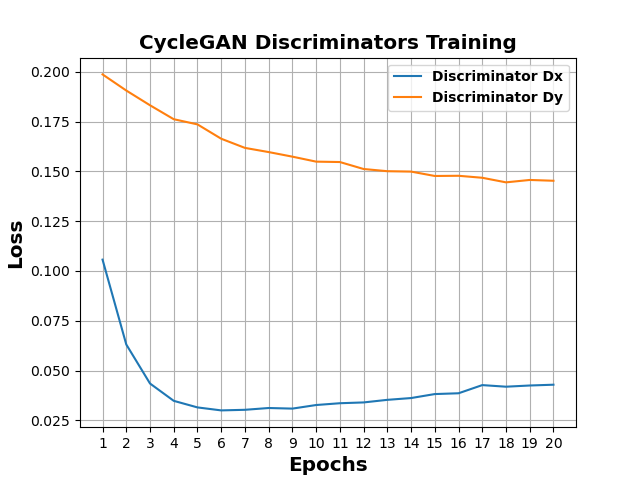
\includegraphics[width=\textwidth]{images/Evaluation/CycleGANDiscriminatorsTraining.png}
    \caption[\ac{CycleGAN} discriminators $D_X$ and $D_Y$ training epochs vs loss plot.]{\ac{CycleGAN} discriminators $D_X$ and $D_Y$ training epochs vs loss plot.}
    \label{fig:CycleGANDiscriminatorsTraining}
  \end{minipage}
\end{figure}

\end{comment}


\section{\ac{GAN} Training}
\vspace*{1.5cm}
\begin{figure}[H]
    \begin{center}
	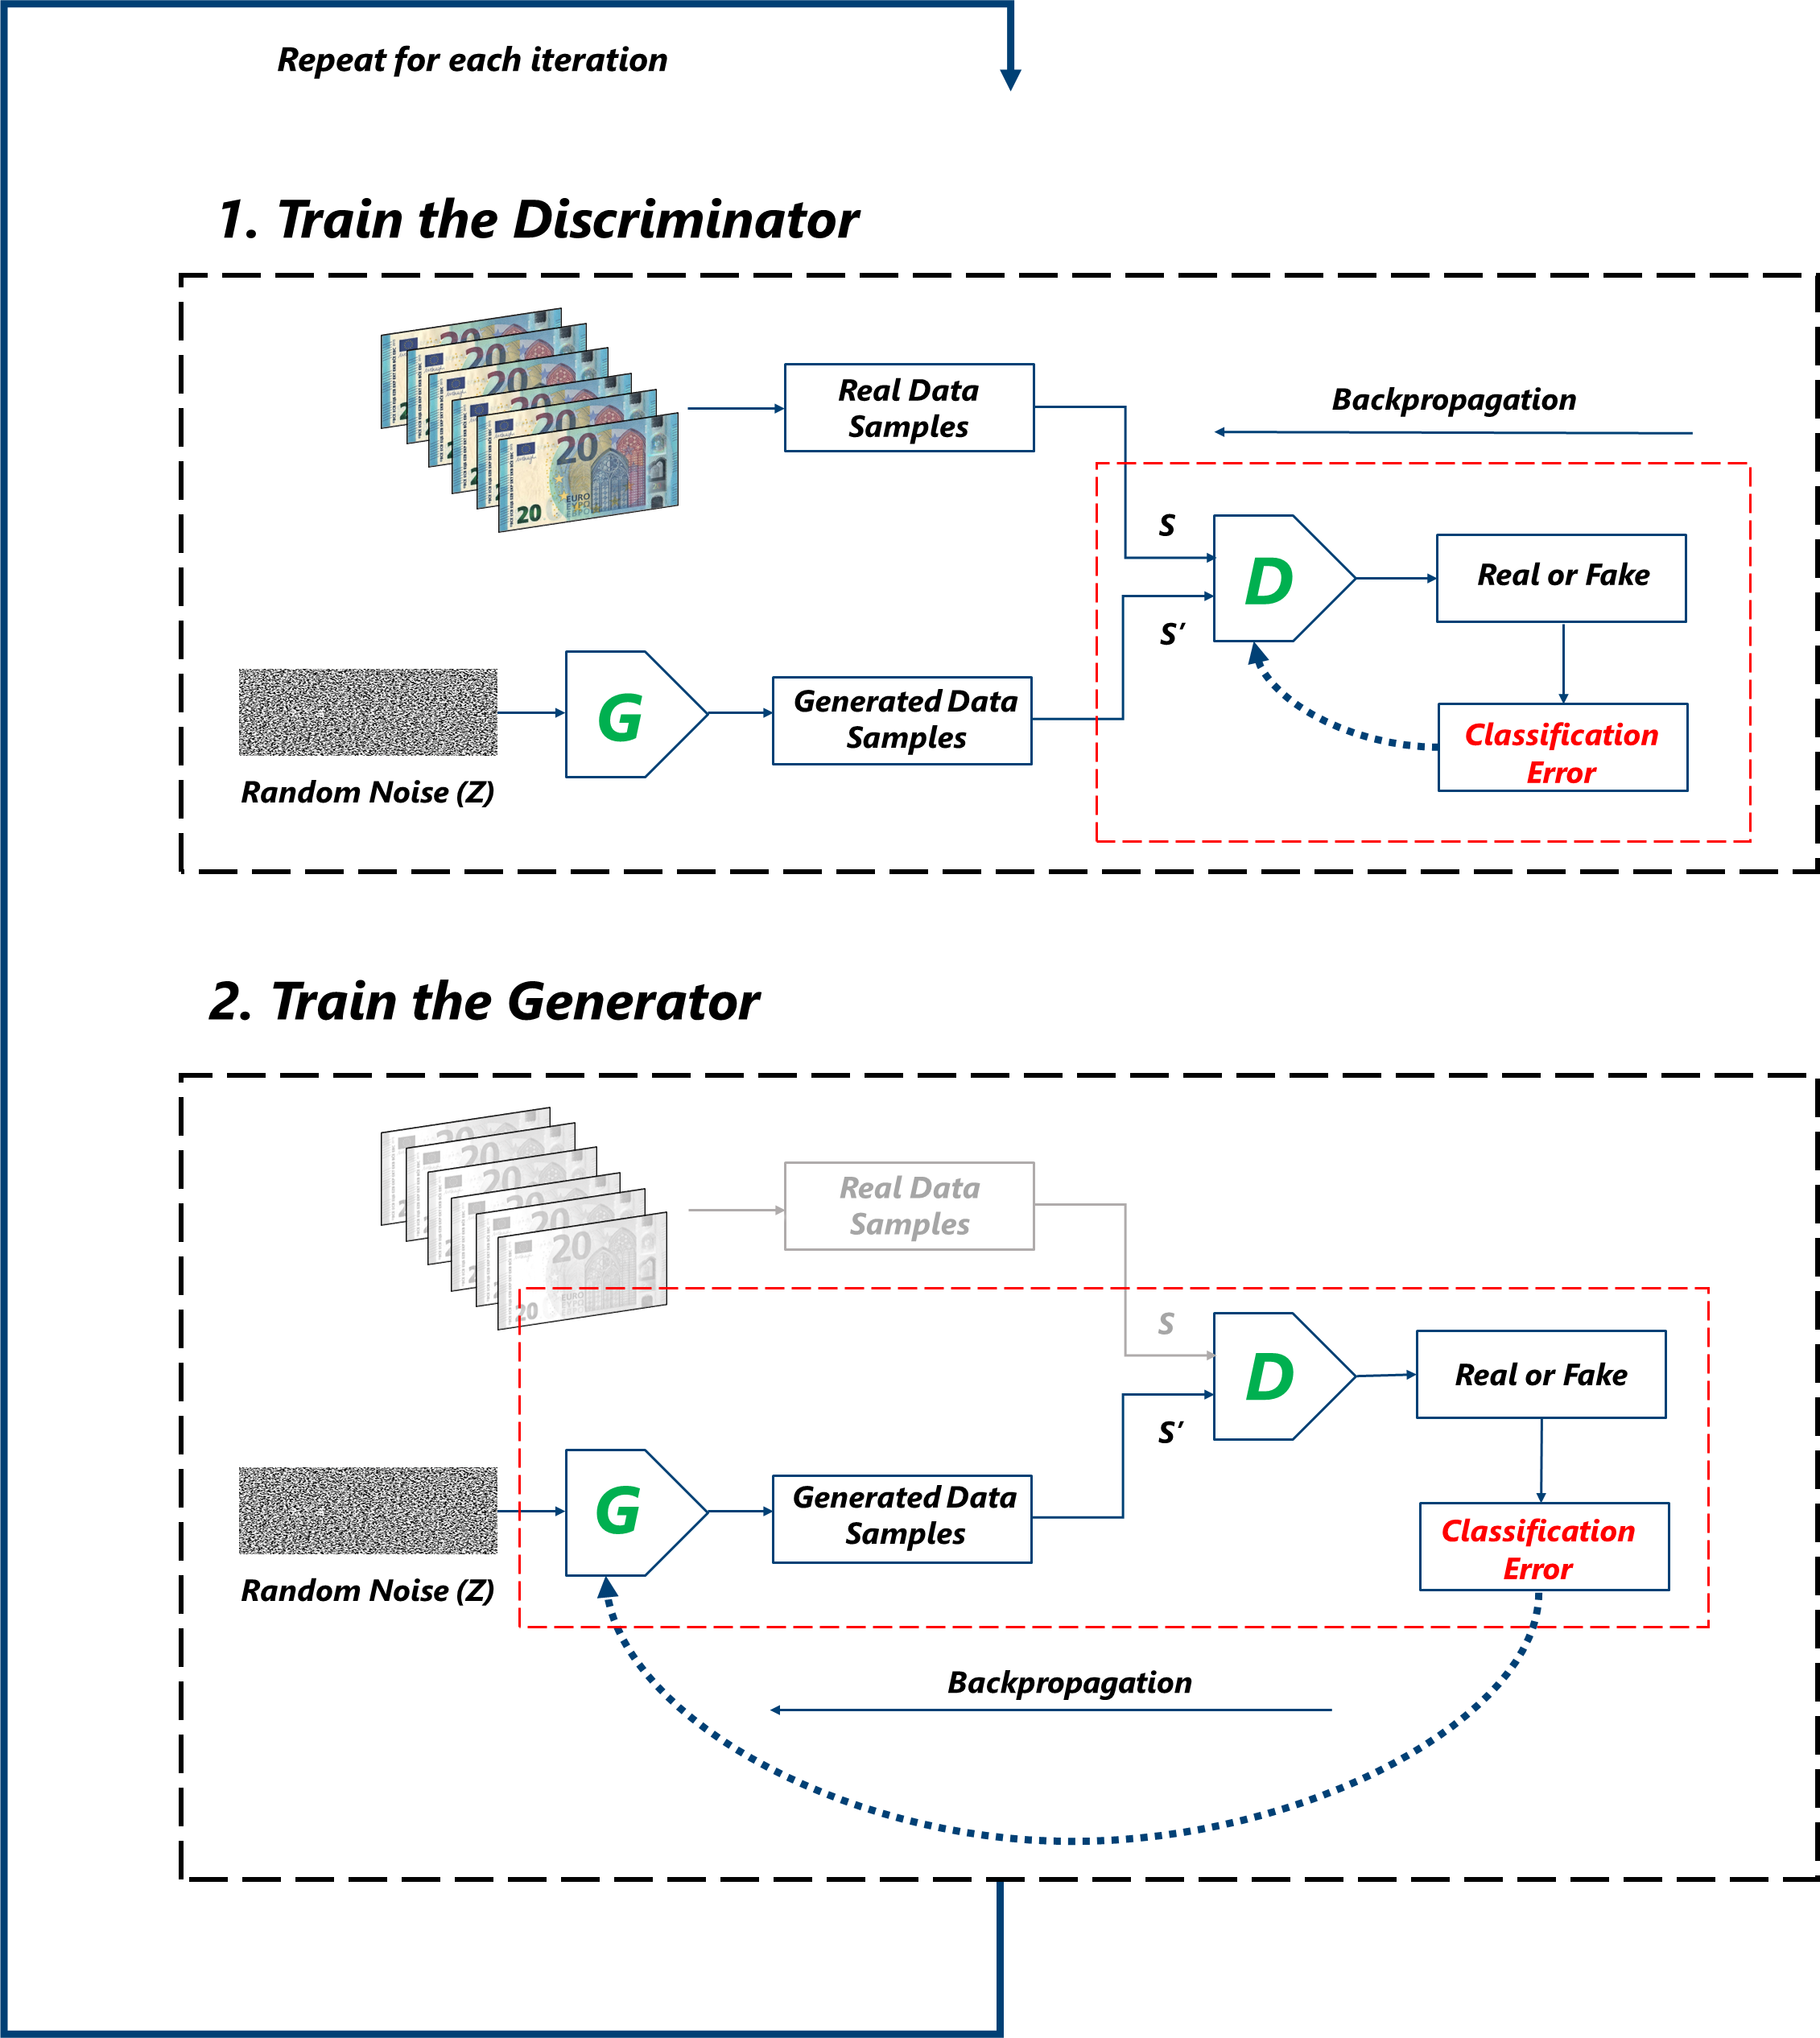
\includegraphics[scale=0.25]{images/Appendix/generatorAndDiscriminatorTraining.png}
	\caption[An illustration of training of the \ac{GAN} as per the algorithm.]{An illustration of training of the \ac{GAN} as per the algorithm.}
	\label{fig:generatorAndDiscriminatorTraining}
	\end{center}
\end{figure}



\section{Examples of Document Images}
\vspace*{0.5cm}
\begin{figure}[H]
        \begin{center}
	    \includegraphics[scale=0.29]{images/Appendix/template.png}
	    \caption[Example of template.]{Examples of template (figure reproduced from elevait GmbH \& Co. KG with permission).}
	    \label{fig:template}
	    \end{center}
\end{figure}

\begin{figure}[H]
        \vspace*{2cm}
        \begin{center}
	    \includegraphics[scale=0.43]{images/Appendix/RealImage.png}
	    \caption[Example of real document image.]{Example of real document image (figure reproduced from elevait GmbH \& Co. KG with permission).}
	    \label{fig:RealImage}
	    \end{center}
\end{figure}

\begin{figure}[H]
        \vspace*{1cm}
        \begin{center}
	    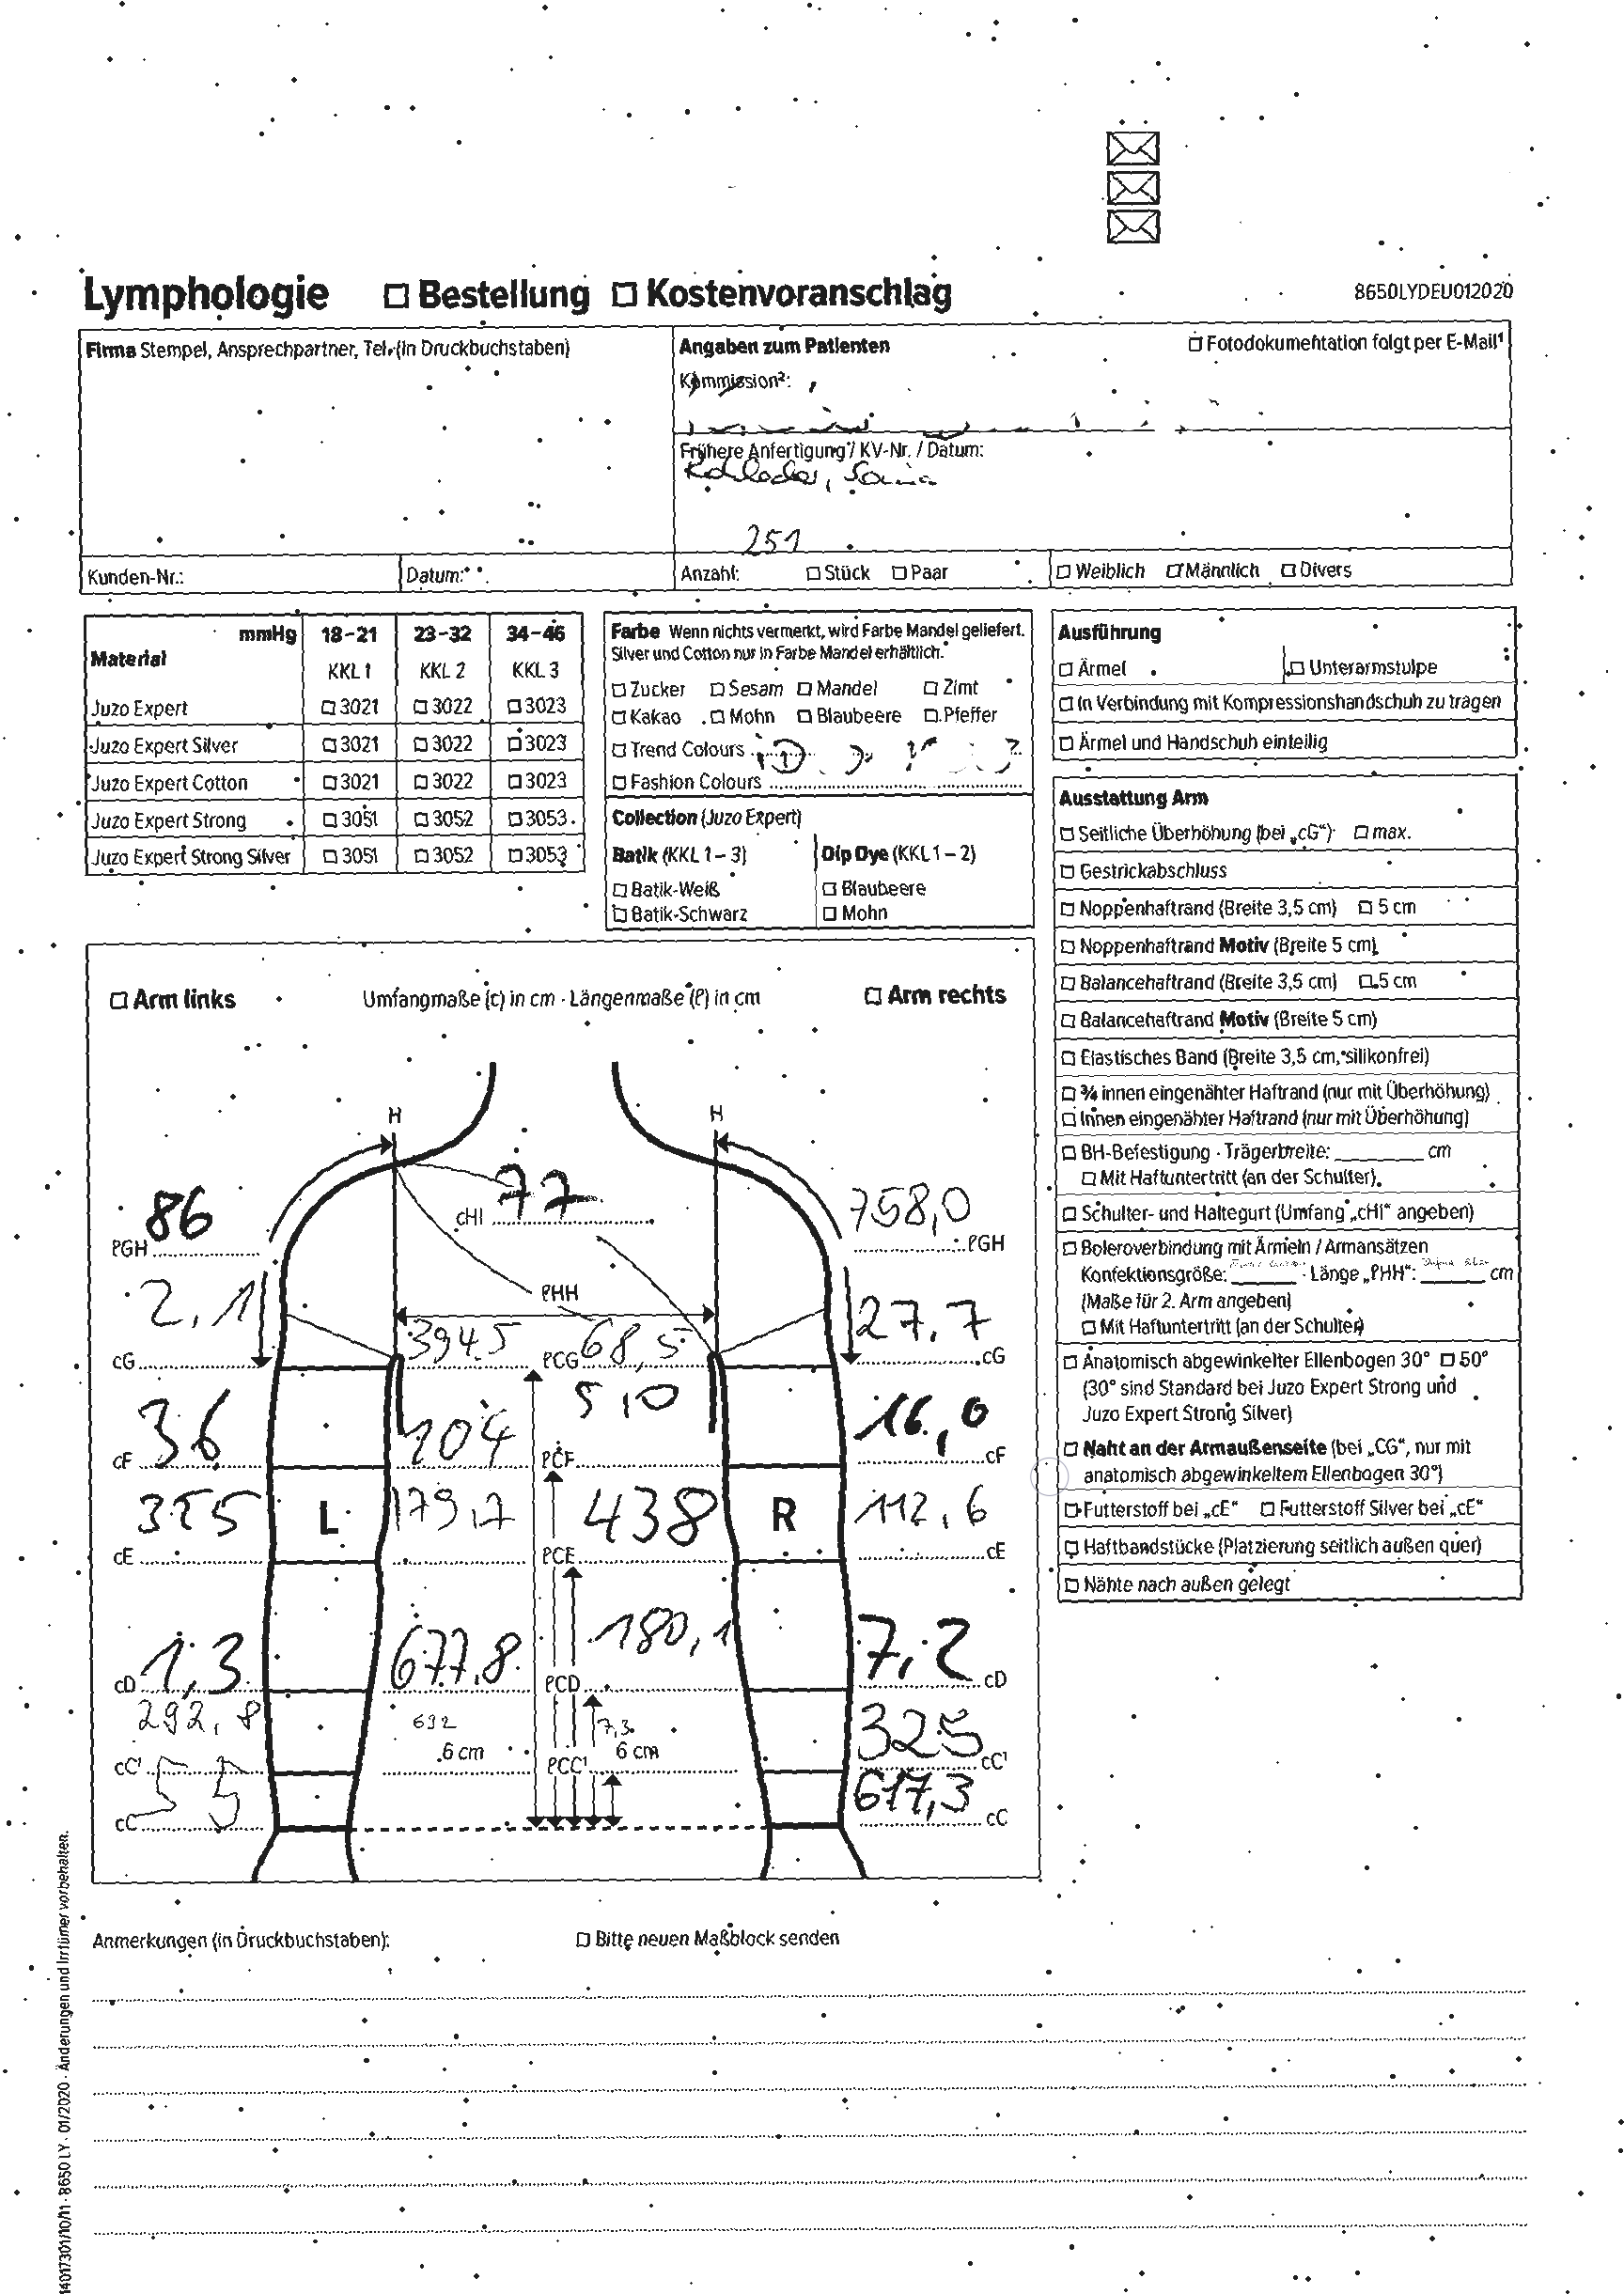
\includegraphics[scale=0.32]{images/Appendix/FaxifiedImage.png}
	    \caption[Examples of faxified document image.]{Examples of faxified document image (figure reproduced from elevait GmbH \& Co. KG with permission).}
	    \label{fig:FaxifiedImage}
	    \end{center}
\end{figure}




\section{Classifier Architecture Diagram}
\begin{figure}[H]
        \vspace*{3cm}
	    \begin{center} 
	    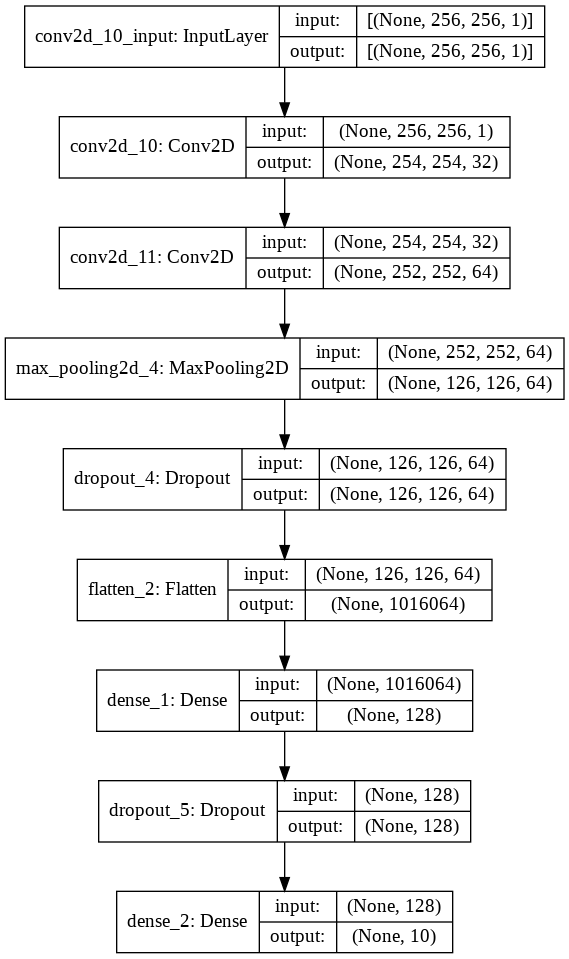
\includegraphics[scale=0.45]{images/Appendix/ClassifierModelSummary.png}
	     \caption{Classifier model summary.}
	     \label{fig:ClassifierModelSummary}
	    \end{center}
\end{figure}


\section{Generator Model Summary}
\vspace*{2.2cm}
\begin{figure}[H]
	    \begin{center} 
	    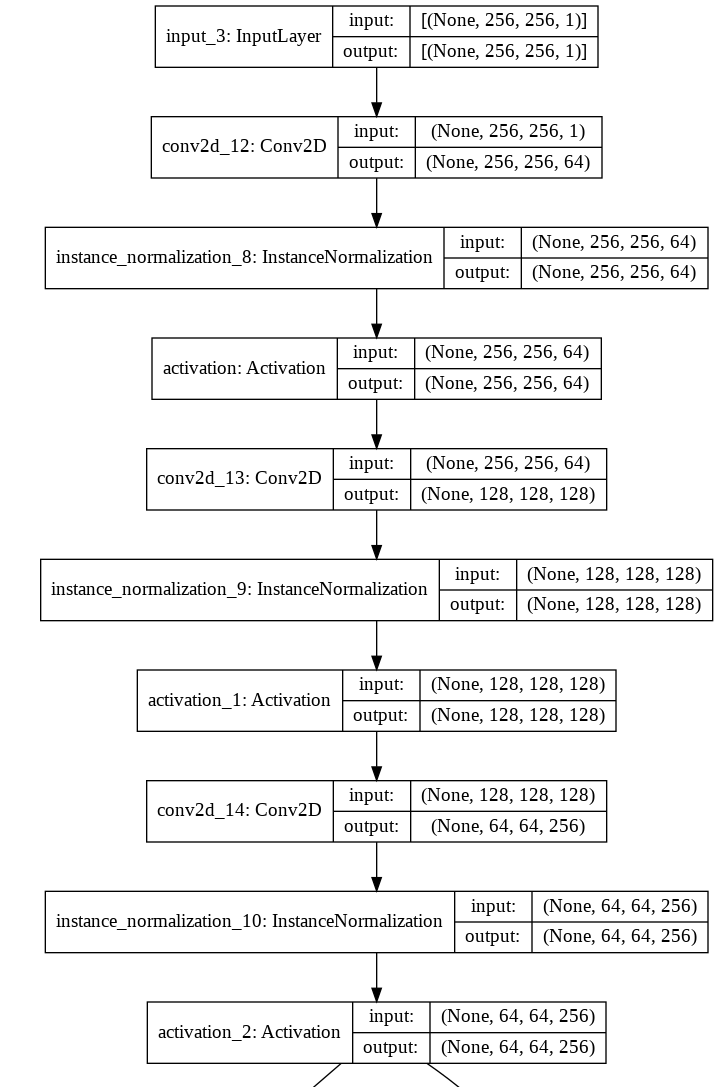
\includegraphics[scale=0.60]{images/Appendix/generator_1.png}
	     \caption{Generator model summary. Continue to next page.}
	     \label{fig:GeneratorModelSummary}
	    \end{center}
\end{figure}


\begin{figure}[H]
        \vspace*{4cm}
	    \begin{center} 
	    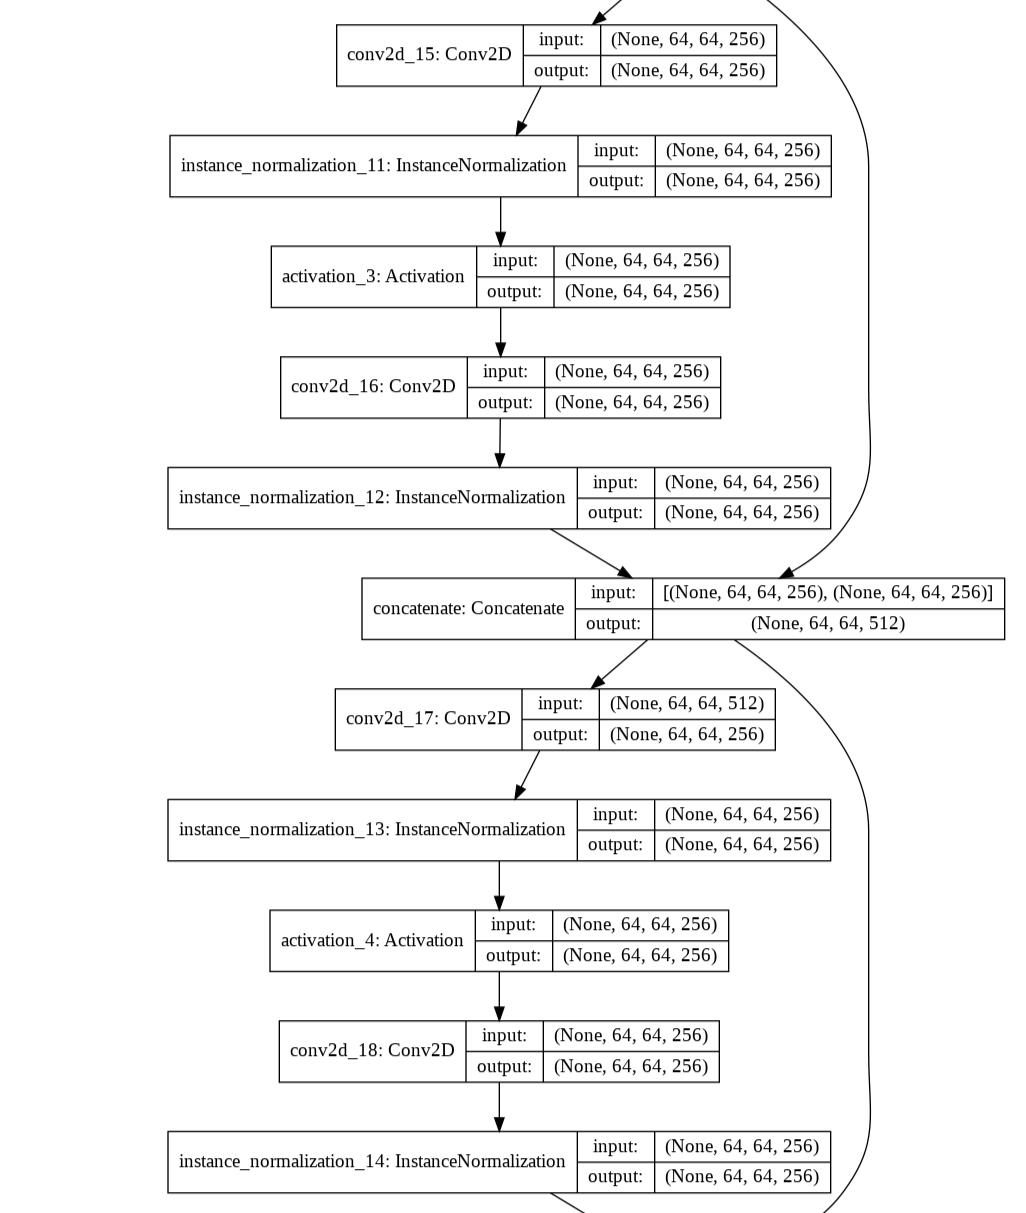
\includegraphics[scale=0.40]{images/Appendix/generator_2.png}
	     \caption{Generator model summary. Continue to next page.}
	    \end{center}
\end{figure}

\begin{figure}[H]
        \vspace*{3cm}
	    \begin{center} 
	    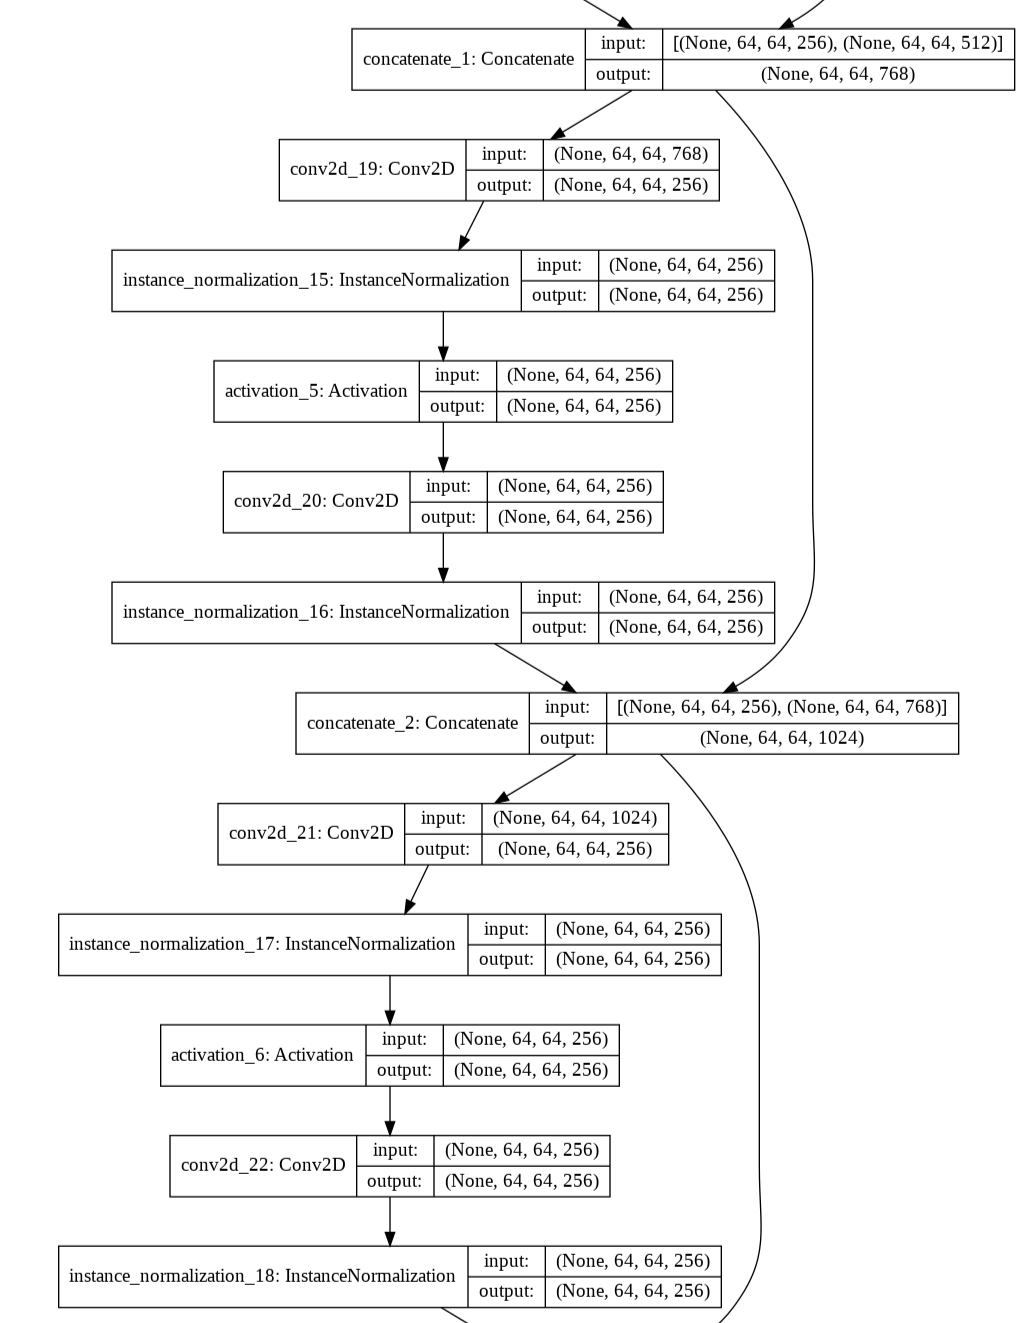
\includegraphics[scale=0.40]{images/Appendix/generator_3.png}
	    \caption{Generator model summary. Continue to next page.}
	    \end{center}
\end{figure}

\begin{figure}[H]
        \vspace*{3cm}
	    \begin{center} 
	    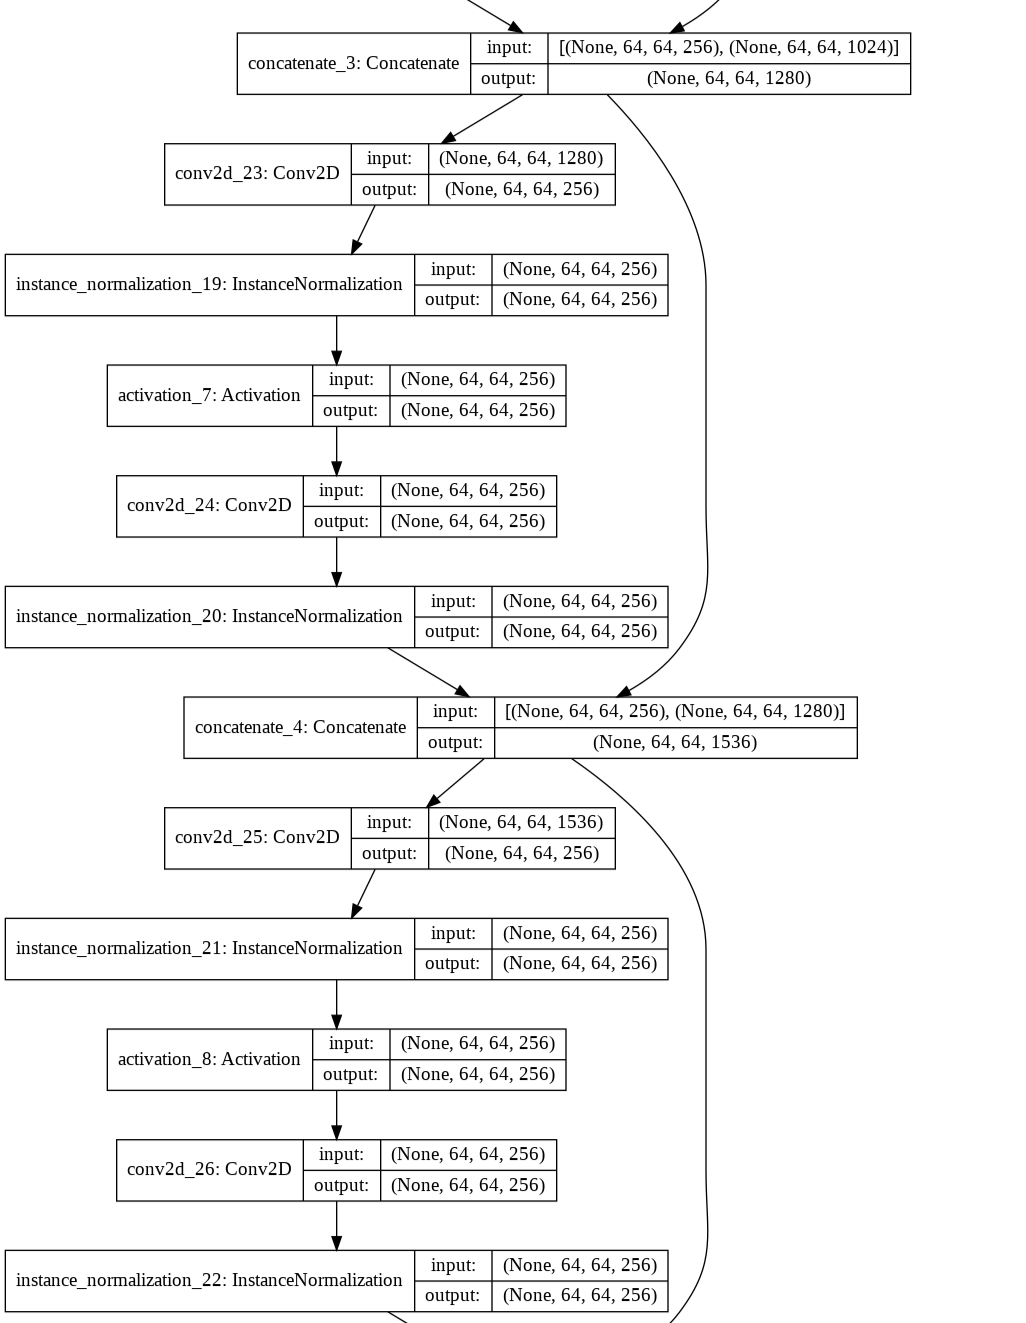
\includegraphics[scale=0.40]{images/Appendix/generator_4.png}
	    \caption{Generator model summary. Continue to next page.}
	    \end{center}
\end{figure}


\begin{figure}[H]
        \vspace*{2cm}
	    \begin{center} 
	    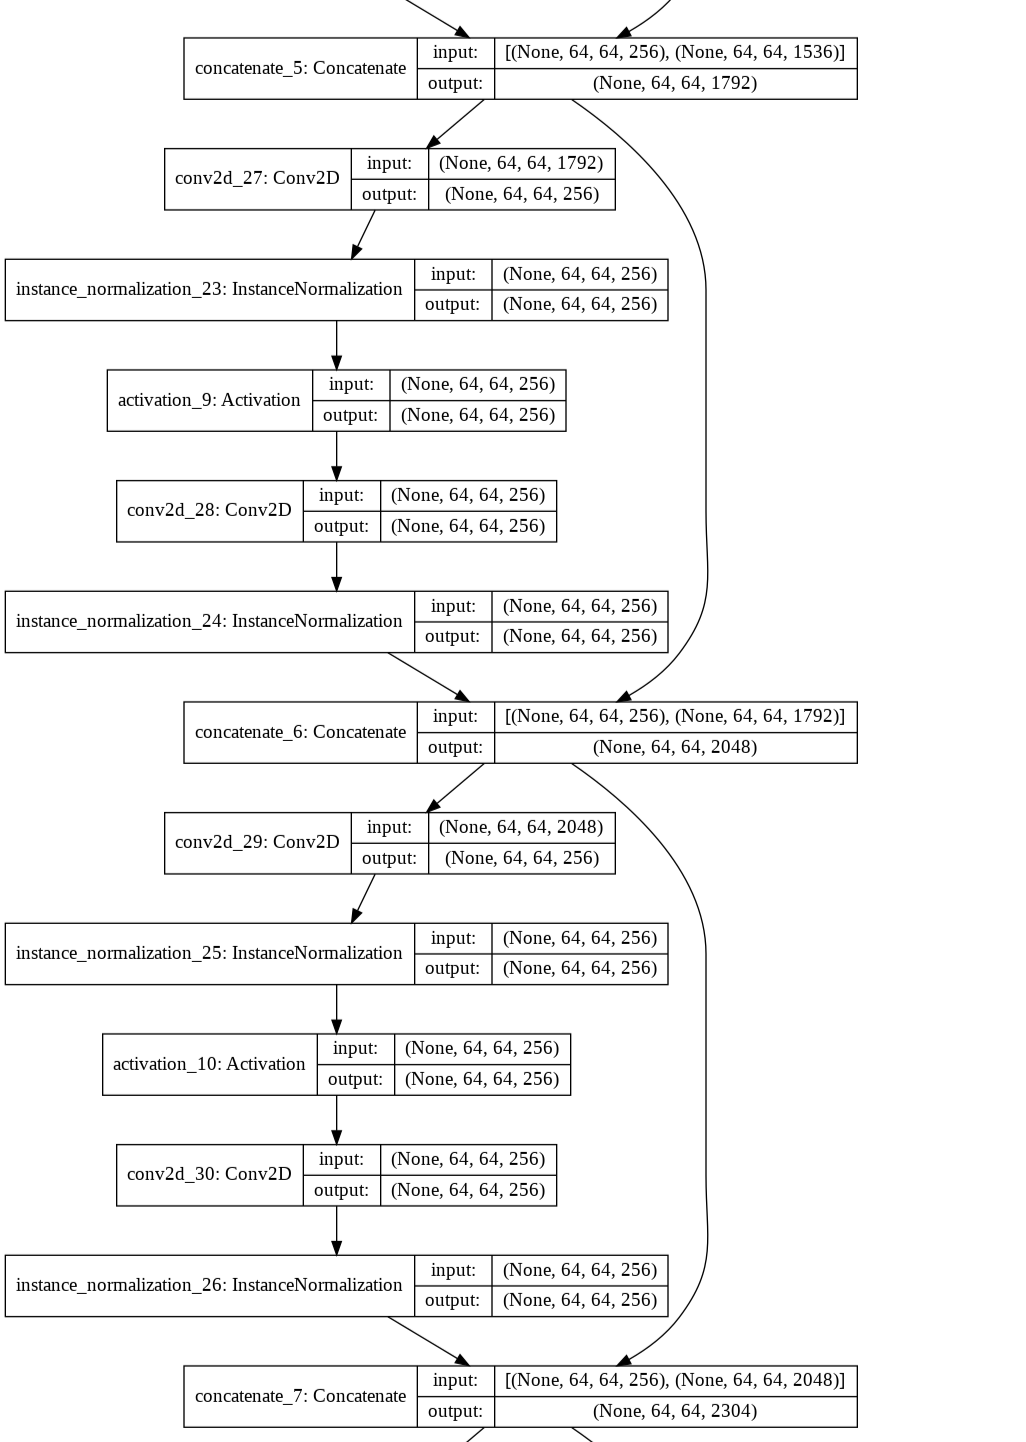
\includegraphics[scale=0.40]{images/Appendix/generator_5.png}
	    \caption{Generator model summary. Continue to next page.}
	    \end{center}
\end{figure}


\begin{figure}[H]
        \vspace*{1cm}
	    \begin{center} 
	    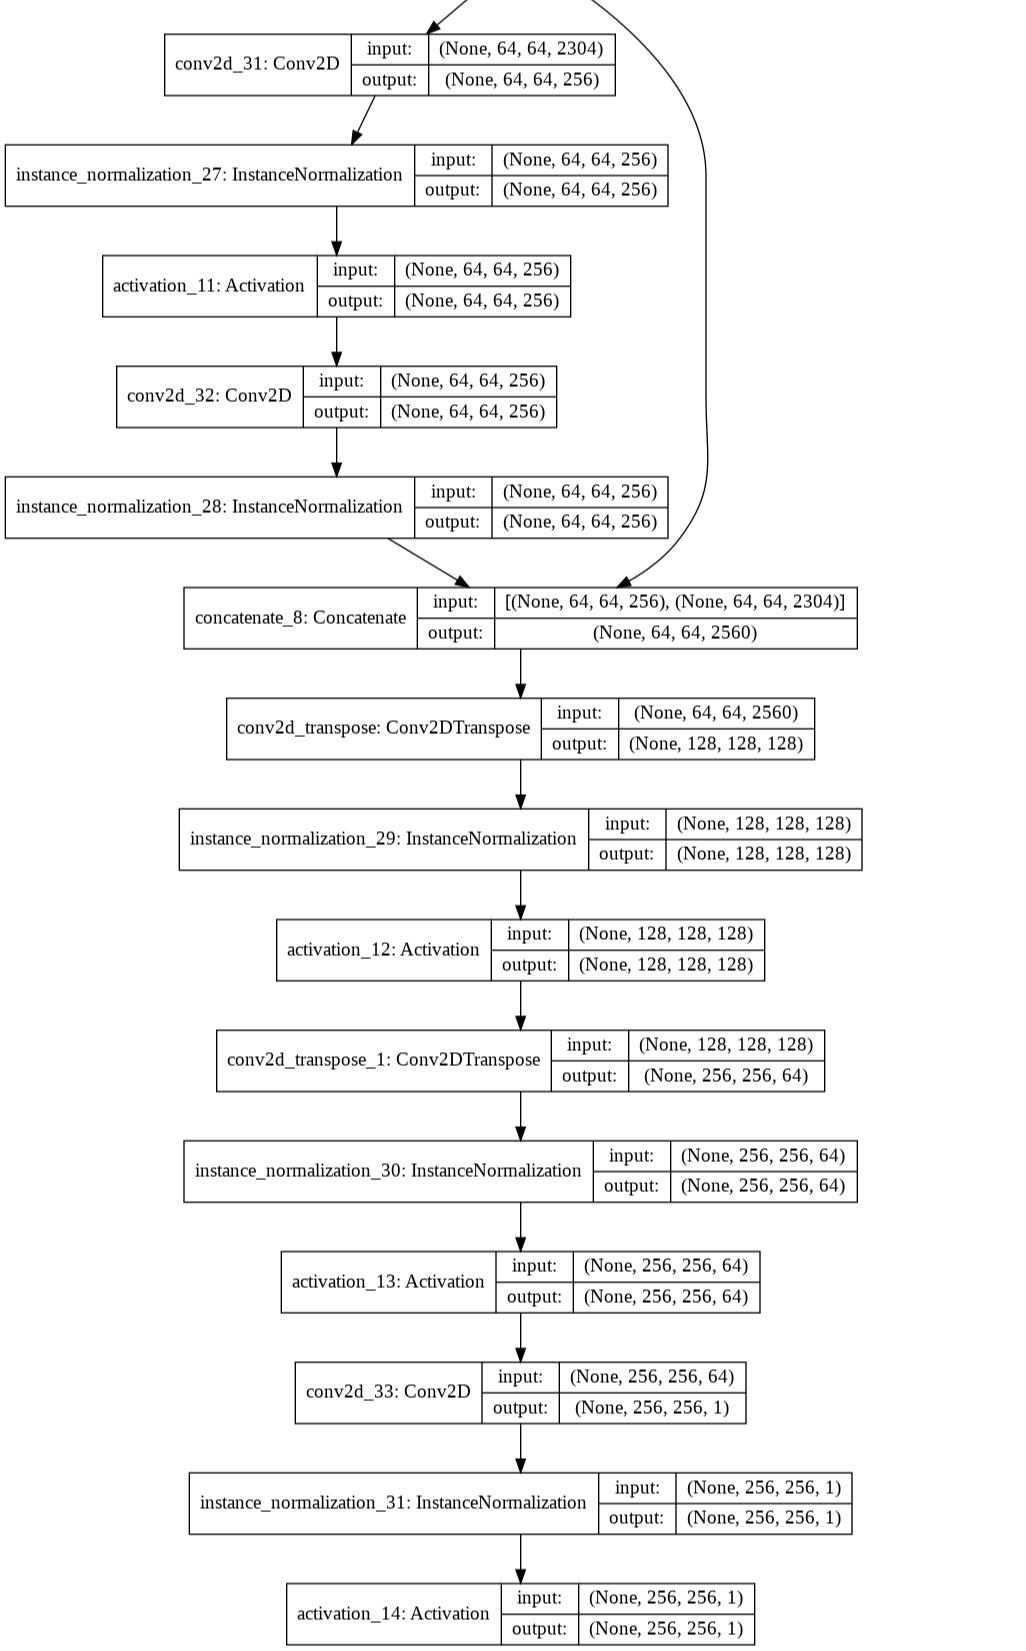
\includegraphics[scale=0.50]{images/Appendix/generator_6.png}
	    \caption{Generator model summary. Ends here.}
	    \end{center}
\end{figure}


\section{Discriminator Model Summary}
\begin{figure}[H]
	    \begin{center} 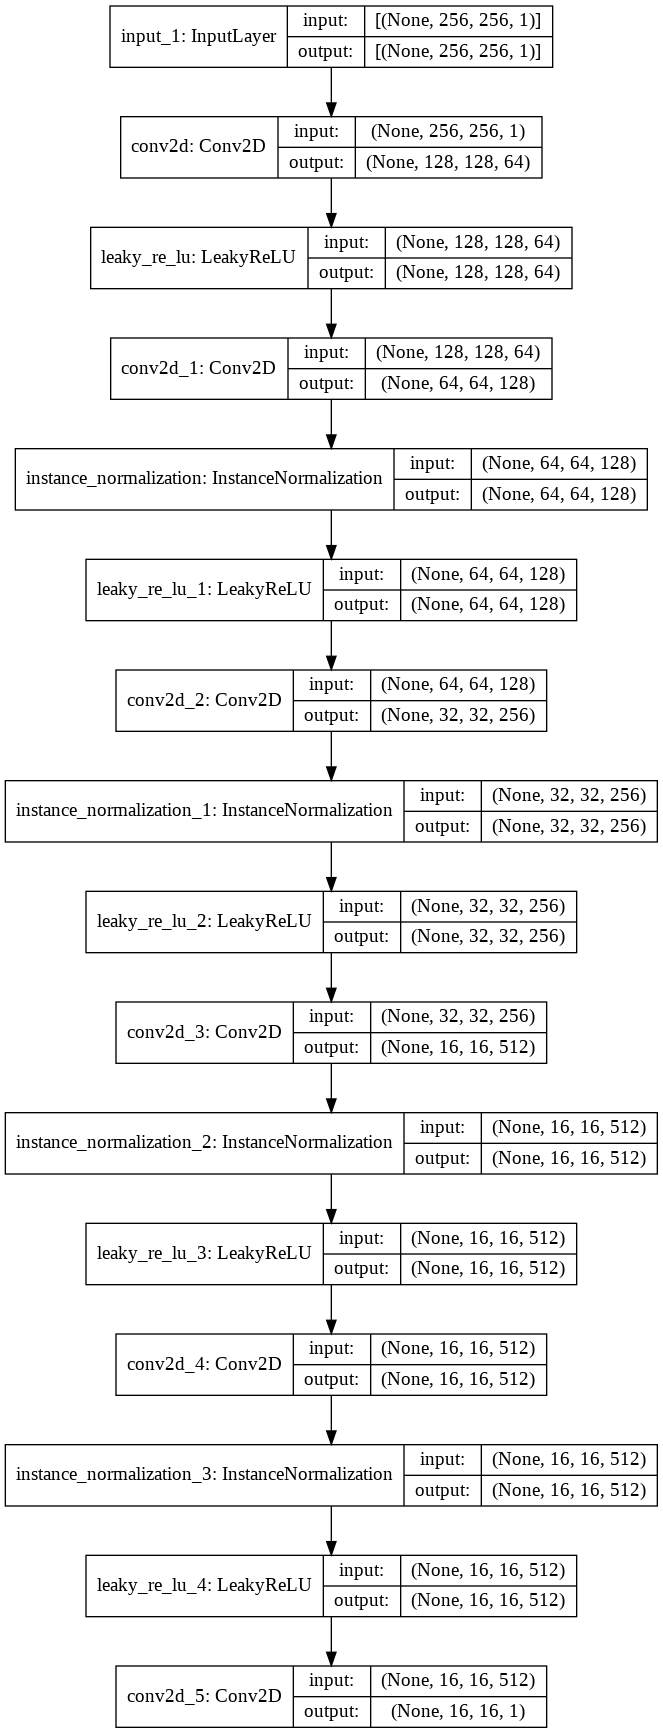
\includegraphics[scale=0.35]{images/Appendix/DiscriminatorModelSummary.png}
	    \caption{Discriminator model summary.}
	    \label{fig:DiscriminatorModelSummary}
	    \end{center}
\end{figure}




%%%%%%%%%%%%%%%%%%%%%%%%%%%%%%%%%%%%%%%%%%%%%%%%%%%%%%%%%%%%%%%%%%%%%%%%%%%%%%%%%%%%%%%%%%%%%%%%%%%%%%%%%%%%%%%


\begin{comment}
\begin{figure}[H]
  \centering
  \begin{minipage}[b]{0.49\textwidth}
    \includegraphics[width=\textwidth]{images/template.png}
    \caption[Sample of template.]{Sample of template.}
    \label{fig:template}
  \end{minipage}
  \hfill
  \begin{minipage}[b]{0.49\textwidth}
    \includegraphics[width=\textwidth]{images/RealImage.png}
    \caption[Sample real document image.]{Sample real document image.}
    \label{fig:RealImage}
  \end{minipage}
\end{figure}


\begin{figure}[H]
  \centering
  \begin{minipage}[b]{0.49\textwidth}
    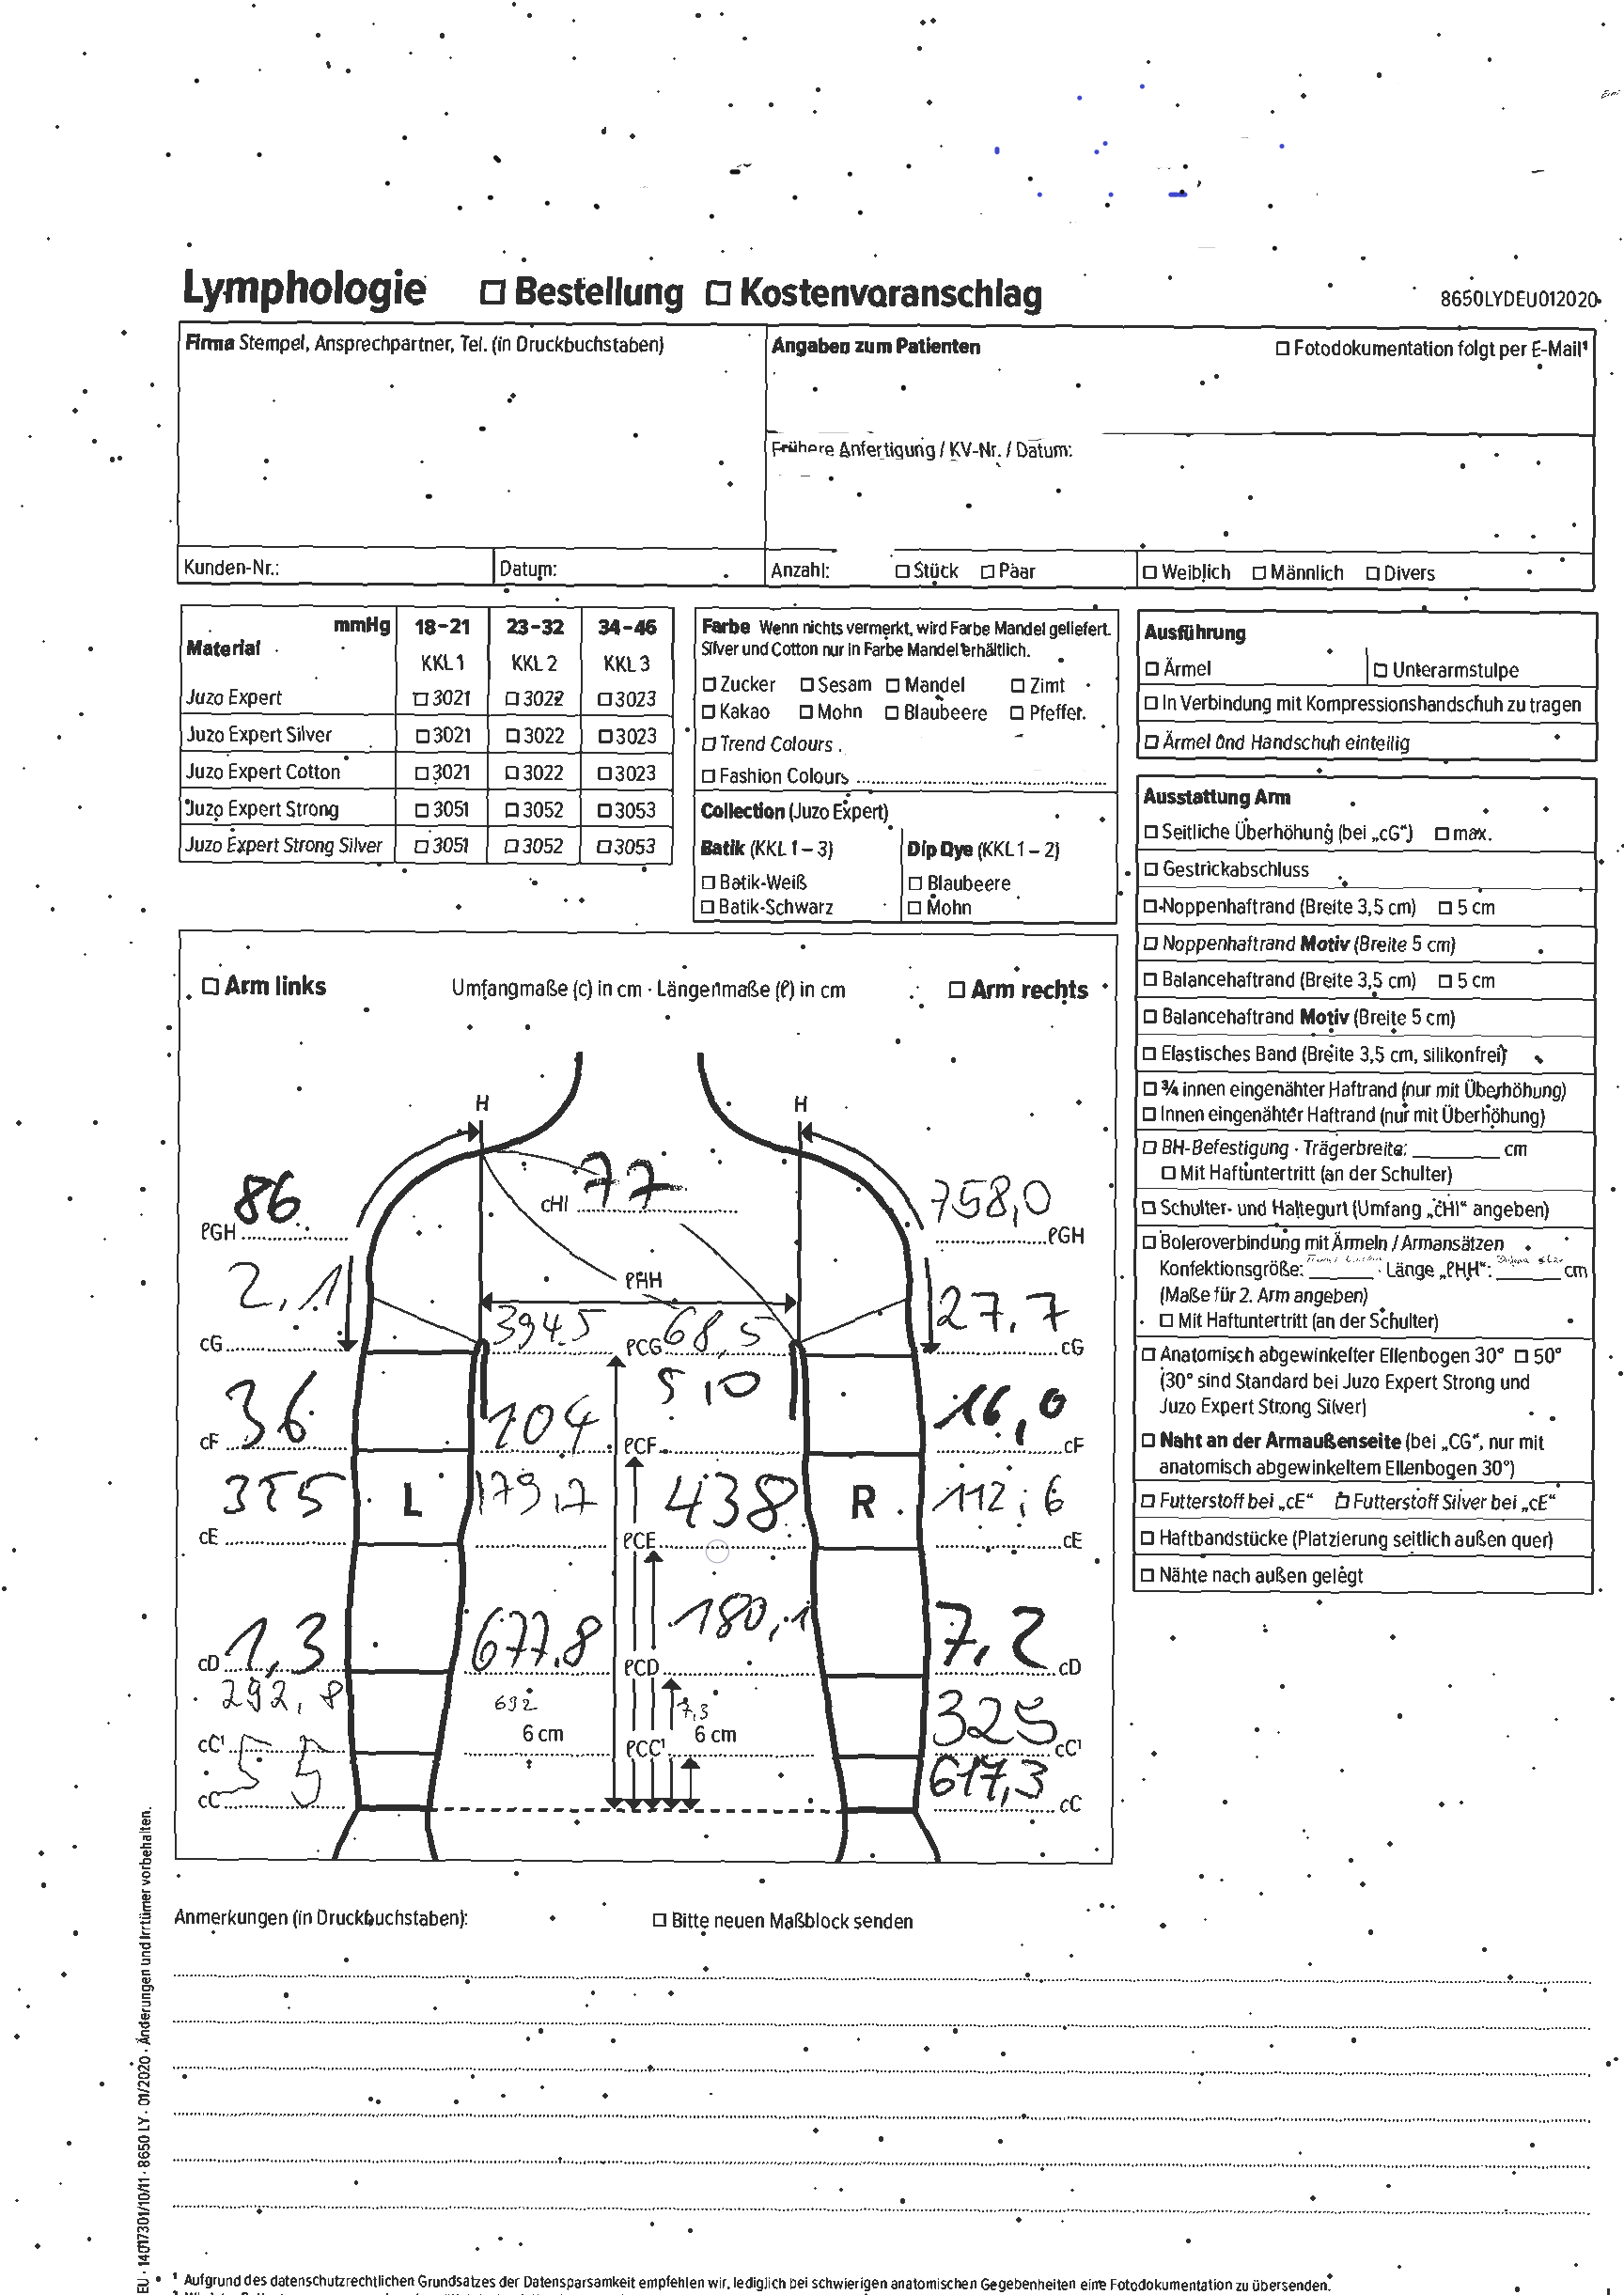
\includegraphics[width=\textwidth]{images/FaxifiedImage.png}
    \caption[Faxified document image.]{Faxified document image.}
    \label{fig:FaxifiedImage}
  \end{minipage}
\end{figure}
\end{comment}


\begin{comment}
\section{Confusion Matrices}

\begin{figure}[H]
  \centering
  \begin{minipage}[b]{0.49\textwidth}
    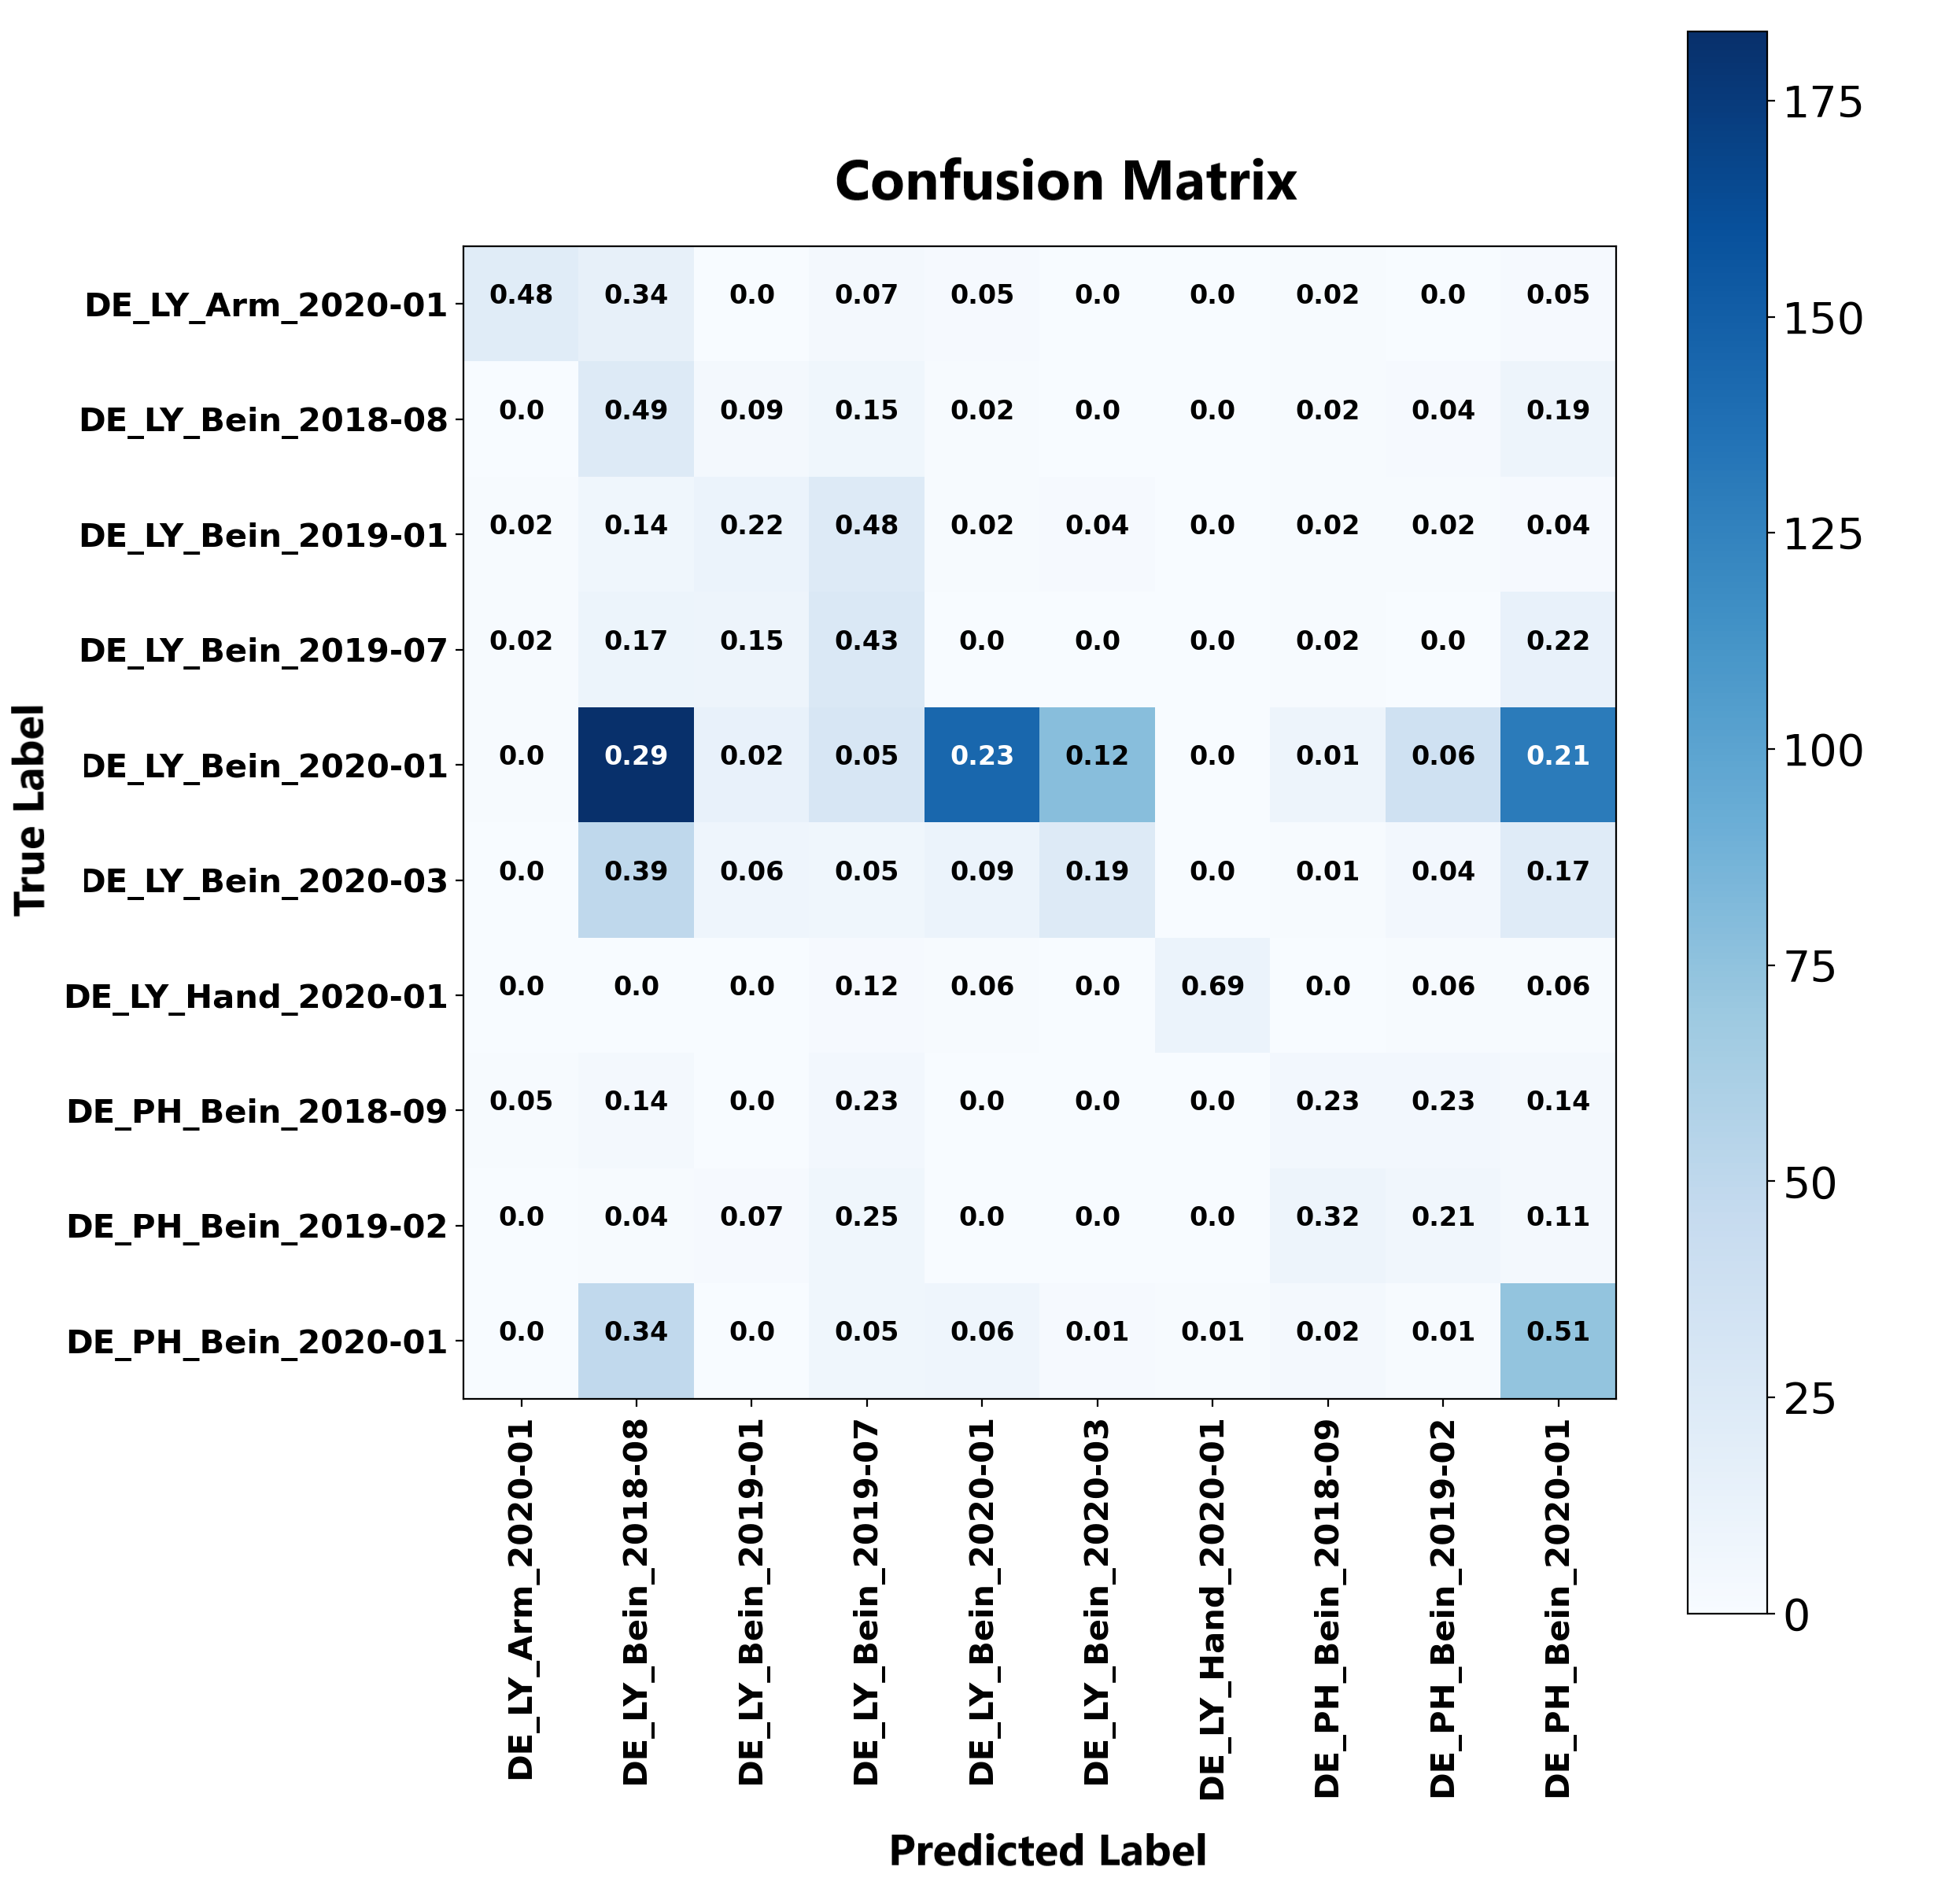
\includegraphics[width=\textwidth]{images/Confusion_Matrix_Synthetic_Data_Classifier_2021-05-21_13-52-04.png}
    \caption[Confustion Matrix. The Classifier Trained On Synthetic Document Images and Evaluated on Real Test Document Images.]{Confustion Matrix. The Classifier Trained on Synthetic Document Images and Evaluated on Real Test Document Images.}
    \label{fig:CMSynthetic}
  \end{minipage}
  \hfill
  \begin{minipage}[b]{0.49\textwidth}
    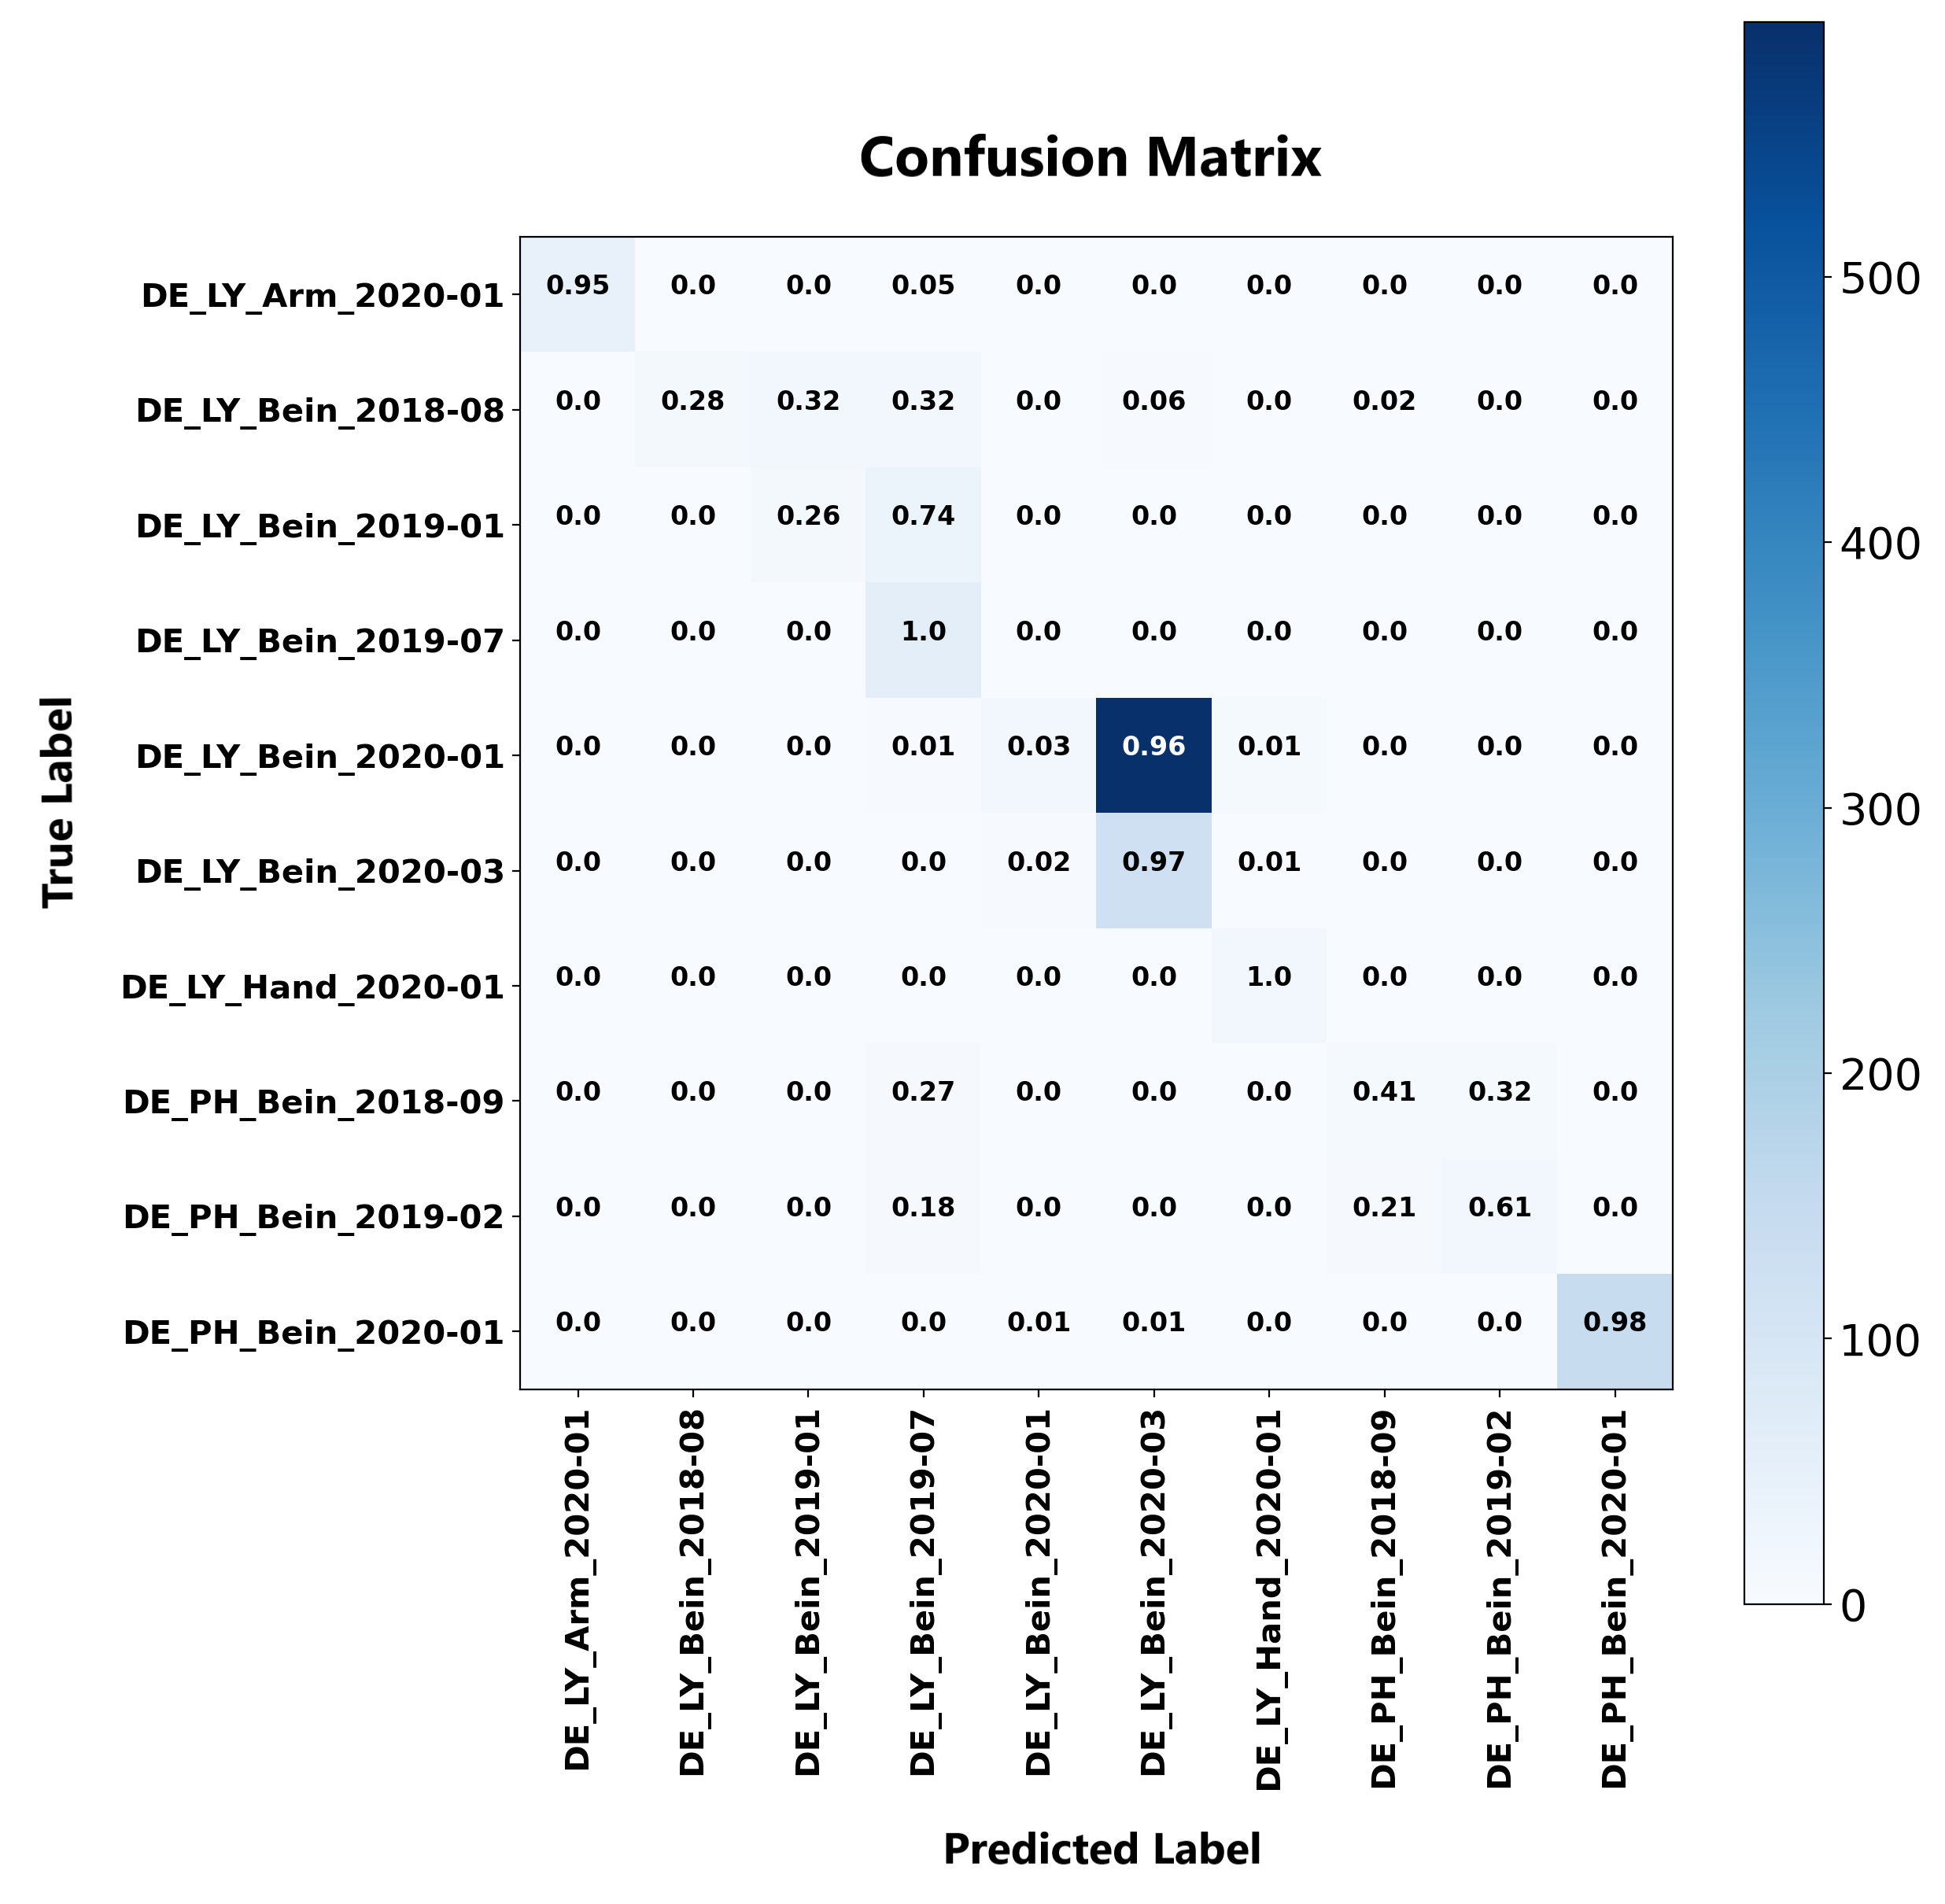
\includegraphics[width=\textwidth]{images/Confusion_Matrix_Faxifier_Data_Classifier_2021-05-21_13-50-07.png}
    \caption[Confustion Matrix. The Classifier Trained On Faxified Document Images and Evaluated on Real Test Document Images.]{Confustion Matrix. The Classifier Trained on Faxified Document Images and Evaluated on Real Test Document Images.}
    \label{fig:CMFaxified}
  \end{minipage}
\end{figure}
\end{comment}


\begin{comment}
\section{\ac{CycleGAN} Training}


\begin{figure}[H]
        \begin{center}
	    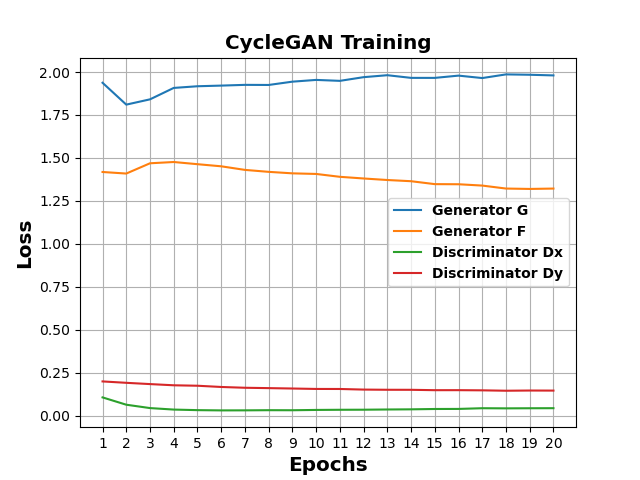
\includegraphics[scale=0.60]{images/CycleGAN_Training.png}
	    \caption[Epoch vs Loss Plot. Training of all the models present in the \ac{CycleGAN}. Generator $G$ and $F$, and Discriminator $D_X$ and $D_Y$.]{Epoch vs Loss Plot. Training of all the models present in the \ac{CycleGAN}Generator $G$ and $F$ and Discriminator $D_X$ and $D_Y$.}
	    \label{fig:CycleGANTraining}
	    \end{center}
\end{figure}
\end{comment}


